\chapter{Desarrollo del proyecto}
\label{chap:desarrollo}

\drop{E}{n} este capítulo se describe el proceso de desarrollo de nuestro sistema de navegación por
satélite. Se empieza enumerando los requisitos originales del sistema y se explica cómo se
realizarán las pruebas. Más tarde se explica iteración a iteración las decisiones tomadas, los
prototipos desarrollados y las pruebas realizadas sobre ellos.

\section{Especificación de requisitos}

Como se comentó anteriormente (ver sección~\ref{sec:metodologia}) los requisitos del sistema se
han ido detallando a lo largo del desarrollo del proyecto ya que, originalmente, sólo teníamos una
idea muy general del sistema a desarrollar. A continuación se muestran estos requisitos generales
sobre los que partimos:

\begin{itemize}
  \item El sistema debe poder guiar a peatones, ciclistas y motoristas.
  \item El sistema debe desplegarse sobre alguna plataforma de \emph{smartphone}.
  \item El sistema debe ser compatible con la mayoría de versiones de la plataforma.
  \item La interacción con el sistema debe desarrollarse de forma implícita y ser válida para
    peatones, ciclistas y motoristas.
  \item En caso de necesitar complementos para la interacción, deben estar disponibles en el
    mercado.
  \item El sistema debe implementar las características básicas del resto de aplicaciones del
    mercado como mostrar la posición en el mapa, rotar el mapa en función de nuestra orientación o
    visualizar la ruta que se va a seguir.
\end{itemize}

\section{Pruebas}

Para describir las pruebas realizadas sobre los diferentes prototipos en este documento se ha
utilizado el patrón «Given-When-Then». Este patrón divide el proceso en 3 etapas:

\begin{itemize}
  \item \textbf{Given} (Dado): Condiciones previas sobre las que se producen los eventos.
  \item \textbf{When} (Cuando): Operaciones específicas que se producen.
  \item \textbf{Then} (Entonces): Resultados esperados.
\end{itemize}

\section{Proceso de desarrollo}

A continuación se indican las iteraciones realizadas durante el desarrollo del \acs{TFG} detallando
los objetivos, el diseño, la implementación y las pruebas de cada una de ellas.

\subsection{Iteración 1: Mostrar mapa}

En la primera iteración nos marcamos como objetivo mostrar una posición cualquiera en el mapa por
medio de una aplicación de \emph{smartphone}.

\subsubsection{Diseño}

Para realizar esta primera aproximación tendremos que tomar tres importantes decisiones de diseño:

\begin{itemize}
  \item Elegir la plataforma de \emph{smartphone} sobre la que desplegar nuestra aplicación.
  \item Elegir el proveedor de mapas que nos proporcionará las imágenes a mostrar.
  \item Elegir la versión objetivo de la plataforma de desarrollo.
\end{itemize}

En primer lugar, tras revisar las diferentes plataformas disponibles para \emph{smartphone} (ver
sección~\ref{sec:plataformas}) se estipuló que la mejor alternativa es Android. Por un lado, Android
posee de la mayor cuota de mercado (81\%) y dispone de una gran variedad de dispositivos en una
amplia gama de precios. Por otro lado, Android es un \acs{SO} que se integra fácilmente con la
plataforma de complementos Android Wear (ver sección~\ref{sec:wearables}) que es la única que nos
permite manipular el vibrador del \emph{wearable} a voluntad.

En segundo lugar, entre los proveedores de mapas existentes (ver sección~\ref{sec:proveedores}) se
seleccionó Open Street Map. Se consideró la mejor elección porque nos provee de mapas de gran
calidad completamente gratuitos. Además, si encontrásemos cualquier tipo de error en los mapas
suministrados, podríamos corregirlo porque es un proyecto colaborativo. Para simplificar el uso de
\acs{OSM} se utilizó la librería \emph{Osmdroid} tal y como se dijo en la
sección~\ref{sec:herramientasSoftware}.

En tercer y último lugar, se seleccionó como objetivo del desarrollo la \acs{API} de Android 21,
también conocida como Android 5.0 \emph{Lollipop}, por ser la más nueva y poseer el mayor número de
funcionalidades. De todos modos, se aseguró la compatibilidad desde la \acs{API} de Android 8,
también llamada Android 2.2 \emph{Froyo}, por medio de la librería \emph{Android support} para
asegurarnos de tener compatibilidad con la mayoría de dispositivos Android.

\subsubsection{Implementación}

Para visualizar los mapas de \acs{OSM} con la ayuda de la librería \emph{Osmdroid} basta con añadir
una vista del tipo \texttt{org.osmdroid.views.MapView} al \texttt{layout} de nuestra aplicación (ver
listado~\ref{code:layoutMapView}) y seleccionar el punto del mapa que deseamos centrar en la
pantalla (ver listado~\ref{code:activityMapView}) por medio de sus coordenadas geográficas.

\begin{listing}[
  float=ht,
  language = xml,
  caption  = {Ejemplo de \texttt{layout} usando \texttt{org.osmdroid.views.MapView}},
  label    = code:layoutMapView]
<?xml version="1.0" encoding="utf-8"?>
<LinearLayout xmlns:android="http://schemas.android.com/apk/res/android"
        xmlns:tools="http://schemas.android.com/tools"
        android:orientation="vertical" 
        android:layout_width="fill_parent"
        android:layout_height="fill_parent">
        
        <org.osmdroid.views.MapView android:id="@+id/map"
                android:layout_width="fill_parent" 
                android:layout_height="fill_parent" />
                
</LinearLayout>
\end{listing}

\begin{listing}[
  float=ht,
  language = java,
  caption  = {Ejemplo de \texttt{activity} mostrando un punto de un mapa en específico},
  label    = code:activityMapView]
public class MainActivity extends Activity {
    @Override
    public void onCreate(Bundle savedInstanceState) {
        super.onCreate(savedInstanceState);
        setContentView(R.layout.main);

        MapView map = (MapView)findViewById(R.id.map);
        map.setMultiTouchControls(true);
        map.getController().setZoom(18);

        GeoPoint startPoint = new GeoPoint(39.40540171, -3.12204771);
        map.getController().setCenter(startPoint);
    }
}
\end{listing}

Por muy sencillo que pueda parecer, durante la implementación detectamos un problema: el mapa no se
centraba en la posición seleccionada. Dejaba dicha posición en la esquina superior izquierda y no en
el centro de la pantalla. Estudiando el problema descubrimos que se trataba de un \emph{bug}
documentado~\footnote{https://github.com/osmdroid/osmdroid/issues/22\#issuecomment-43092313} de
\emph{Osmdroid} y que se resolvería en la próxima versión de la librería.

Para paliar dicho problema, y siguiendo con las instrucciones detalladas en el \emph{bug},
procedimos a implementar un método que lo resolviera (ver listado~\ref{code:centerMap}).

\begin{listing}[
  float=ht,
  language = java,
  caption  = {Método utilizado para centrar el mapa en cualquier posición},
  label    = code:centerMap]
private void centerMap(final GeoPoint loc) {
    mMap.getViewTreeObserver().addOnGlobalLayoutListener(
            new ViewTreeObserver.OnGlobalLayoutListener() {
        @Override
        public void onGlobalLayout() {
            mMap.getViewTreeObserver().removeGlobalOnLayoutListener(this);
            mMap.getController().setCenter(loc);
        }
    });
}
\end{listing}

\subsubsection{Pruebas}

Al finalizar la implementación del primer prototipo se realizó la siguiente prueba:

\begin{itemize}
  \item Para determinar la correcta carga de los mapas en diferentes localizaciones

  \begin{tabular}{p{.15\textwidth}p{.75\textwidth}}
    \hline
    \textbf{Dado}     & Diferentes coordenadas geográficas \\
                      & Diferentes dispositivos con distintas versiones de Android (ver
                        sección~\ref{sec:herramientasHardware}) \\
    \textbf{Cuando}   & Ejecutamos la aplicación \\
    \textbf{Entonces} & Se muestra dicha ubicación centrada en un mapa \\
    \hline
  \end{tabular}
\end{itemize}

\subsection{Iteración 2: Mostrar posición actual en el mapa}

Una vez evaluado el prototipo de la iteración 1, se procedió a añadir una nueva funcionalidad:
mostrar la posición actual en la aplicación.

\subsubsection{Diseño}

Para poder mostrar la ubicación actual, es necesario primero conocerla. Para ello, analizamos en la
sección~\ref{sec:tecnologiasActuales} los diferentes sistemas con los que podemos obtener nuestras
coordenadas geográficas en la actualidad. Puesto que \acs{GLONASS} no estuvo operativo para uso
civil hasta 2012 no todos los \emph{smartphones} disponen en la actualidad de esta tecnología y nos
deja con una única opción razonable: \acs{NAVSTAR-GPS}.

\subsubsection{Implementación}

Para hacer uso del \acs{GPS} de nuestro \emph{smartphone} en Android sólo es necesario definir un
\texttt{LocationListener} e indicar por medio de un \texttt{LocationManager} qué clase lo implementa
y cada cuanto tiempo queremos que se ejecute (ver listado~\ref{code:locationManager}).

\begin{listing}[
  float=ht,
  language = java,
  caption  = {Ejemplo de uso de \texttt{LocationManager} utilizando la propia clase como
                 \texttt{LocationListener} y 1 segundo de intervalo entre actualizaciones},
  label    = code:locationManager]
if (mLocationManager.isProviderEnabled(LocationManager.GPS_PROVIDER)) {
    mLocationManager.requestLocationUpdates(LocationManager.GPS_PROVIDER, 1000, 1, this);
}
\end{listing}

Para que una clase implemente un \texttt{LocationListener} debe contener cuatro funciones:

\begin{itemize}
  \item \textbf{\texttt{onLocationChanged}} Para indicar qué hacer cuando nuestra ubicación cambia.
  \item \textbf{\texttt{onProviderDisabled}} Para indicar qué hacer cuando se desactiva el
    \acs{GPS}.
  \item \textbf{\texttt{onProviderEnabled}} Para indicar qué hacer cuando se activa el \acs{GPS}.
  \item \textbf{\texttt{onStatusChanged}} Para indicar qué hacer cuando cambia el estado del
    proveedor del servicio \acs{GPS}. Los posibles estados son \emph{fuera de servicio},
    \emph{temporalmente no disponible} y \emph{disponible}.
\end{itemize}

Resulta obvio que sólo necesitamos rellenar el método \texttt{onLocationChanged} con el código
necesario para mostrar una señal en el mapa (ver listado~\ref{code:onLocationChanged}). Para
simplificar la forma de dibujar nuestra posición en el mapa y mostrar el error cometido por la
trilateración (ver sección~\ref{fig:trilateracion}) de forma visual, se ha escrito una clase llamada
\texttt{LocationOverlay} en base a la clase contenida en \emph{Osmbonuspack} (ver
sección~\ref{sec:herramientasSoftware}) con el mismo nombre. Lo único verdaderamente significativo
que diferencia ambas clases es el icono utilizado para especificar nuestra posición en el mapa.

\begin{listing}[
  float=ht,
  language = java,
  caption  = {Ejemplo de implementación de \texttt{LocationListener} utilizando para mostrar la
                localización un \texttt{LocationOverlay}},
  label    = code:onLocationChanged]
public void onLocationChanged(Location loc) {
    GeoPoint myLocation = new GeoPoint(loc); 	
    
    if (!mLocationOverlay.isEnabled()) {
        mLocationOverlay.setEnabled(true);
    }
    mLocationOverlay.setLocation(myLocation);
    mLocationOverlay.setAccuracy((int)loc.getAccuracy());

    centerMap(myLocation);
}
\end{listing}

\subsubsection{Pruebas}

Al finalizar la implementación del segundo prototipo se realizó la siguiente prueba:

\begin{itemize}
  \item Para determinar la correcta carga de los mapas en diferentes localizaciones

  \begin{tabular}{p{.15\textwidth}p{.75\textwidth}}
    \hline
    \textbf{Dado}     & Diferentes localizaciones geográficas \\
                      & Diferentes dispositivos con distintas versiones de Android (ver
                        sección~\ref{sec:herramientasHardware}) \\
    \textbf{Cuando}   & Ejecutamos la aplicación \\
    \textbf{Entonces} & Se muestra dicha ubicación centrada en un mapa \\
    \hline
  \end{tabular}
\end{itemize}

\subsection{Iteración 3: Orientar mapa}

Una vez evaluado el prototipo de la iteración 2 se introdujo una nueva funcionalidad: rotar el mapa
en función de nuestra orientación. Si por ejemplo caminamos por una calle recta en dirección Oeste,
en la pantalla se vería una recta vertical. De igual manera, si por ejemplo caminamos por una calle
en dirección Sur y giramos hacia el Este, en la pantalla se vería un giro a la izquierda.

\subsubsection{Diseño}

Para poder rotar el mapa en función de nuestra orientación es necesario conocer dónde se encuentran
cualquiera de los puntos cardinales: Norte, Sur, Este u Oeste.

Prácticamente todos los \emph{smartphones} actuales disponen de un componente llamado \emph{sensor
  de orientación} que nos permite determinar la orientación espacial del teléfono por medio de tres
valores expresados en grados:

\begin{itemize}
  \item \textbf{Roll} Mide la inclinación del móvil en ralación a los laterales. Desde -90º con el
    lateral izquierdo levantado, hasta 90º con el lateral derecho levantado.
  \item \textbf{Pitch} Mide la inclinación del móvil en relación a la parte anterior y
    posterior. Desde -90º que corresponde a la posición vertical, hasta los 90º que corresponde con
    la parte anterior del móvil, pasando por 0º cuando el teléfono se encuentra a nivel.
  \item \textbf{Azimuth} Mide el punto cardinal Norte en sentido horario de 0º a 360º
\end{itemize}

\subsubsection{Implementación}

Para hacer uso del sensor de orientación de nuestro \emph{smartphone} Android basta con registrar el
uso del \texttt{Sensor} de orientación por medio de un \texttt{SensorManager} (ver
listado~\ref{code:orientacion}) indicando que clase implementa los métodos necesarios para manejar
el sensor de orientación. En este caso la propia (\texttt{this}).

\begin{listing}[
  float=ht,
  language = java,
  caption  = {Ejemplo de registro de un \texttt{Sensor} de orientación con \texttt{SensorManager}},
  label    = code:orientacion]
mSensorManager = (SensorManager) getSystemService(Context.SENSOR_SERVICE);
mOrientation = mSensorManager.getDefaultSensor(Sensor.TYPE_ORIENTATION);
mSensorManager.registerListener(this, mOrientation, SensorManager.SENSOR_DELAY_NORMAL);
\end{listing}

El sensor de orientación en Android obliga a implementar en una clase dos métodos:

\begin{itemize}
  \item \textbf{\texttt{onSensorChanged}} Para definir qué hacer cuando cambie algún valor en el
    sensor. En el caso del sensor de orientación, proporcionará dichos valores en un \texttt{array}
    con tres posiciones:
    \begin{itemize}
      \item \textbf{Posición 0} Para los grados \texttt{azimuth}.
      \item \textbf{Posición 1} Para los grados \texttt{pitch}.
      \item \textbf{Posición 2} Para los grados \texttt{roll}.
    \end{itemize}
  \item \textbf{\texttt{onAccuracyChanged}} Para definir qué hacer cuando cambien la precisión del
    sensor.
\end{itemize}

Para implementar nuestra rotación de mapa bastó con implementar el método \texttt{onSensorChanged} y
pasar al mapa dicha rotación (ver listado~\ref{code:accuracyChanged}).

\begin{listing}[
  float=ht,
  language = java,
  caption  = {Ejemplo de rotación de mapa en función del sensor de orientación},
  label    = code:accuracyChanged]
public void onSensorChanged(SensorEvent event) {
    float azimuth = event.values[0];
    mMap.setMapOrientation(-azimuth);
}
\end{listing}

\subsubsection{Pruebas}

Al finalizar la implementación del tercer prototipo se realizaron las siguiente pruebas:

\begin{itemize}
  \item Para comprobar la correcta orientación del mapa

  \begin{tabular}{p{.15\textwidth}p{.75\textwidth}}
    \hline
    \textbf{Dado}     & Aplicación ejecutándose mientras se camina en dirección Norte \\
                      & Diferentes dispositivos con distintas versiones de Android (ver
                        sección~\ref{sec:herramientasHardware}) \\
    \textbf{Cuando}   & Se gira al Oeste o al Este \\
    \textbf{Entonces} & Se muestra un giro a la izquierda y derecha respectivamente \\
    \hline
  \end{tabular}

  \begin{tabular}{p{.15\textwidth}p{.75\textwidth}}
    \hline
    \textbf{Dado}     & Aplicación ejecutándose mientras se camina en dirección Sur \\
                      & Diferentes dispositivos con distintas versiones de Android (ver
                        sección~\ref{sec:herramientasHardware}) \\
    \textbf{Cuando}   & Se gira al Oeste o al Este \\
    \textbf{Entonces} & Se muestra un giro a la derecha e izquierda respectivamente \\
    \hline
  \end{tabular}
\end{itemize}

\subsection{Iteración 4: Crear y mostrar ruta}

Una vez evaluado el prototipo de la iteración 3, se procedió a añadir una nueva funcionalidad: crear
rutas para peatones, ciclistas o motoristas desde nuestra posición actual hasta una determinada
localización geográfica (latitud y longitud) y dibujarla en el mapa.

\subsubsection{Diseño}

Para poder calcular una ruta tenemos que hacer uso de alguno de los proveedores vistos en la
sección~\ref{sec:proveedores}. Puesto que se optó por usar los mapas de \acs{OSM} y ya tenemos
importadas las librerías \emph{Osmdroid} y \emph{Osmbonuspack} que nos permiten calcular rutas para
peatones, ciclistas y motorias; la opción más lógica es utilizar \emph{MapQuest}.

\subsubsection{Implementación}

Para la creación y superposición en el mapa de una ruta utilizando \emph{Osmdroid} y
\emph{Osmbonuspack} basta con indicar el tipo de usuario, el punto de inicio de la ruta y de
finalización. Con esta información, realiza una consulta en Internet a la \acs{API} de
\emph{MapQuest}~\footnote{http://wiki.openstreetmap.org/wiki/MapQuest} y nos devuelve una ruta
específica que solo resta dibujar en el mapa (ver listado~\ref{code:gotov1}).

\begin{listing}[
  float=ht,
  language = java,
  caption  = {Ejemplo de creación y superposición de una ruta en el mapa},
  label    = code:gotov1]
private Boolean gotoGeoPoint(GeoPoint endPoint) {
    RoadManager roadManager = new MapQuestRoadManager(MAPQUESTAPIKEY);
    roadManager.addRequestOption("units=k");
    roadManager.addRequestOption("routeType=fastest");
    //roadManager.addRequestOption("routeType=shortest");
    //roadManager.addRequestOption("routeType=bicycle");
    //roadManager.addRequestOption("routeType=pedestrian");
    
    ArrayList<GeoPoint> waypoints = new ArrayList<GeoPoint>();
    waypoints.add(getLastLocation());
    waypoints.add(endPoint);
    
    mRoad = roadManager.getRoad(waypoints);
            
    mRoadOverlay = RoadManager.buildRoadOverlay(road, getBaseContext());
    mRoadOverlay.setWidth(10);

    mMap.getOverlays().add(mRoadOverlay);            
    mMap.invalidate();
}
\end{listing}

Pero existe un problema con el listado~\ref{code:gotov1}: Cuando utilizamos como objetivo de
desarrollo una \acs{API} de Android superior a 9, no realiza la petición a Internet y nos muestra
una línea recta entre el origen y el destino. Este \emph{bug} esta documentado en
\emph{Osmbonuspack}~\footnote{https://code.google.com/p/osmbonuspack/issues/detail?id=9} aunque no
sea culpa de la librería.

El problema radica en la forma que realizamos la petición a Internet. Desde la \acs{API} de Android
10 y posteriores, Google decidió que realizar peticiones a Internet en el mismo \emph{thread} en
el que se ejecuta la \acf{GUI} era un error. Lo estimó así porque podía provocar la sensación de que
la aplicación no funciona cuando lo que verdaderamente está ocurriendo es que se encuentra esperando
una respuesta de Internet.

Por tanto, para que nuestras rutas funcionen sólo podemos realizar dos acciones:

\begin{itemize}
  \item Eliminar las políticas de \emph{threads} (ver listado~\ref{code:threads}) y seguir usando el
    mismo código.
  \item Utilizar un \emph{thread} diferente al de la \acs{GUI} para realizar la petición a Internet.
    (ver listado~\ref{code:gotov2}.
\end{itemize}


\begin{listing}[
  float=ht,
  language = java,
  caption  = {Eliminación de políticas de threads},
  label    = code:threads]
StrictMode.ThreadPolicy policy = new StrictMode.ThreadPolicy.Builder().permitAll().build();
StrictMode.setThreadPolicy(policy);
\end{listing}

\begin{listing}[
  float=ht,
  language = java,
  caption  = {Ejemplo de creación y superposición de una ruta en el mapa utilizando una
                 \texttt{AsyncTask}},
  label    = code:gotov2]
private void gotoGeoPoint(GeoPoint endPoint) {
    ArrayList<GeoPoint> waypoints = new ArrayList<GeoPoint>();
    waypoints.add(getLastLocation());
    waypoints.add(endPoint);
  
    new GetRoad().execute(waypoints);
}

private class GetRoad extends AsyncTask<ArrayList<GeoPoint>, Float, Boolean>{
    protected Boolean doInBackground(ArrayList<GeoPoint>... params) {
        RoadManager roadManager = new MapQuestRoadManager(MAPQUESTAPIKEY);
        roadManager.addRequestOption("units=k");
        roadManager.addRequestOption("routeType=" + mTransport);
      
        mRoad = roadManager.getRoad(params[0]);
      
        return true;
    }
    protected void onPostExecute(Boolean result) {
        if (result) gotoGeoPointPosThread();
  }
  
private void gotoGeoPointPosThread() {
    mRoadOverlay = RoadManager.buildRoadOverlay(mRoad, getBaseContext());
    mRoadOverlay.setWidth(10);
  
    mMap.getOverlays().add(mRoadOverlay);
    mMap.invalidate();
}
\end{listing}

Para implementarlo en nuestro sistema, se seleccionó la segunda opción porque se consideró que se
trataba de la forma correcta de hacerlo y se añadieron algunas animaciones (no incluidas en el
listado~\ref{code:gotov2}) para la espera en la recepción de la ruta.

\subsubsection{Pruebas}

Al finalizar la implementación del cuarto prototipo se realizó la siguiente prueba:

\begin{itemize}
  \item Para comprobar el correcto cálculo de rutas para diferentes usuarios y destinos

  \begin{tabular}{p{.15\textwidth}p{.75\textwidth}}
    \hline
    \textbf{Dado}     & Diferentes perfiles de usuarios: peatones, ciclistas y motoristas \\
                      & Diferentes coordenadas de destinos \\
                      & Diferentes dispositivos con distintas versiones de Android (ver
                        sección~\ref{sec:herramientasHardware}) \\
    \textbf{Cuando}   & Llamamos al método \texttt{gotoGeoPoint} \\
    \textbf{Entonces} & Observamos en el mapa la ruta desde nuestra localización hasta las
                        coordenadas elegidas teniendo en cuenta nuestro método de desplazamiento \\
    \hline
  \end{tabular}
\end{itemize}

\subsection{Iteración 5: Navegar por ruta}

Una vez evaluado el prototipo de la iteración 4, se procedió a añadir una nueva funcionalidad:
navegar por la ruta creada en la iteración anterior observando los mensajes suministrados por el
\emph{smartphone}.

\subsubsection{Diseño}

Para diseñar esta nueva funcionalidad se tuvieron en cuenta tres factores:

\begin{itemize}
  \item La \textbf{velocidad} a la que nos desplazamos. Hay que tener en cuenta que, cuando estamos
    usando la aplicación, el tiempo con el que nos tienen que avisar para realizar una acción
    variará en función de la velocidad que llevemos. Aprovechando este punto, también incorporaremos
    una mejora visual que tienen la mayoría de aplicaciones de navegación: cambiaremos el
    \emph{zoom} del mapa en función de la velocidad que llevemos para que no se sufran grandes
    cambios en el mapa cuando circulamos a una velocidad elevada.

  \item Cómo \textbf{detectamos si se sigue la ruta marcada}. Hay que tener en cuenta que sólo
    disponemos de nuestras coordenadas geográficas y de las coordenadas del siguiente punto a
    alcanzar. Si implementamos un algoritmo en el que consideramos que podemos pasar a la siguiente
    etapa cuando lleguemos a la que estamos realizando, es posible que no funcione. Por ejemplo, si
    nos acercamos a una etapa de \emph{girar a la derecha} y giramos en el sitio correcto antes de
    que la aplicación detecte que hemos llegado (probablemente por la precisión de los satélites
    \acs{GPS}), no cargaría la siguiente etapa y no sabríamos qué está sucediendo.

  \item El posible \textbf{desvío de la ruta establecida}. Hay que plantearnos cómo detectar que nos
    hemos salido de la ruta marcada y qué hacer en esos casos. Al tratarse de una aplicación de
    navegación diseñada para que ella interactúe con nosotros y no al contrario, la opción más
    interesante es que, cuando detecte nuestro desvío, nos avise y nos calcule una nueva ruta desde
    la posición en la que nos encontramos.

\end{itemize}

\subsubsection{Implementación}

Las tres implementaciones antes descritas, se llevarán a cabo dentro del método
\texttt{onLocationChanged} que ya comenzamos a escribir en la iteración 2. Se debe realizar en éste
método porque, tal y como lo tenemos configurado en el \texttt{LocationManager} (ver
listado~\ref{code:locationManager}), se ejecutará cada segundo con los nuevos datos suministrados
por los satélites \acs{GPS}:

\begin{itemize}
  \item En función de la \textbf{velocidad} que llevemos, se consideraron validos los valores de
    cercanía y \emph{zoom} reflejados en el listado~\ref{code:velocidad}.

    \begin{listing}[
      float=ht,
      language = java,
      caption  = {Ejemplo de implementación de \texttt{LocationListener} utilizado para variar el
                  zoom del mapa y determinar la distancia necesaria para avisar de las acciones},
      label    = code:velocidad]
public void onLocationChanged(Location loc) {  
  [...]
    
  float speed = loc.getSpeed();
  int metersToFirstWarning;

  if (speed > kmhToMs(100)) {
      mMap.getController().setZoom(15);
      metersToFirstWarning = 1000;
  } else if (speed > kmhToMs(80)) {
      mMap.getController().setZoom(16);
      metersToFirstWarning = 500;
  } else if (speed > kmhToMs(50)) {
      mMap.getController().setZoom(17);
      metersToFirstWarning = 100;
  } else if (speed > kmhToMs(20)) {
      mMap.getController().setZoom(18);
      metersToFirstWarning = 60;
  } else {
      mMap.getController().setZoom(18);
      metersToFirstWarning = 30;
  }
    \end{listing}

  \item Para \textbf{detectar si seguimos la ruta marcada} se ha implementado el algoritmo del
    listado~\ref{code:sigueRuta}. El algoritmo indica la acción de \emph{seguir recto} hasta que la
    distancia hasta la próxima etapa es menor que la distancia del comienzo de los avisos del punto
    anterior. Es entonces cuando:

    \begin{itemize}
      \item Si nos acercamos, se nos muestra la etapa a realizar.
      \item Si nos alejamos, se considera que hemos superado la etapa a realizar. De este modo,
        pasamos a la siguiente etapa, a menos que nos encontremos en la última y finalicemos la
        navegación.
    \end{itemize}

    \begin{listing}[
      float=ht,
      language = java,
      caption  = {Ejemplo de implementación de \texttt{LocationListener} utilizado para seguir una
                 ruta almacenada en \texttt{mRoad}},
      label    = code:sigueRuta]
private Boolean mNewAction = true;
private int mStep = 0;
private float mMetersToGoal = Float.MAX_VALUE;

public void onLocationChanged(Location loc) {
  GeoPoint myLocation = new GeoPoint(loc);
  
  [...]

  if (mRoad != null) {
    float distance = getDistance(myLocation, mRoad.mNodes.get(mStep).mLocation);
      
    if (distance < metersToFirstWarning) {
      if (distance < mMetersToGoal) {
        if (mNewAction || mMetersToGoal == Float.MAX_VALUE) {
          mNewAction = false;
          startAction(getAction(mRoad.mNodes.get(mStep).mManeuverType), distance);
        }
        mMetersToGoal = distance;
      } else {
        mNewAction = true;
        mMetersToGoal = Float.MAX_VALUE;
            
        if (mStep == mRoad.mNodes.size()-1) {
          cleanMap();  //Finished
        } else {
          mStep++;
        }
      }
    } else {
      if (mNewAction) {
        mNewAction = false;
        startAction(STRAIGHT, distance);
      }
    }
  }
    \end{listing}

  \item Para detectar cuándo nos \textbf{desviamos de la ruta establecida} hemos utilizado una
    función de la clase \texttt{RoadOverlay} que nos indica en píxeles a cuanta distancia se
    encuentra un punto de una ruta (ver listado~\ref{code:desvio}). Puesto que la ruta va a tener siempre la misma anchura en
    píxeles nos acerquemos o nos alejemos de ella con el \emph{zoom} y nuestro
    \texttt{LocationOverlay} también (24 píxeles), con éste método podremos determinar cuándo nos
    hemos desviado y también podremos apreciarlo en el mapa.

    Además para prevenir posibles errores puntuales en la localización, para considerar un desvío de
    ruta, hemos implementado un contador de errores y sólo se vuelve a calcular el recorrido una vez
    que se ha detectado 3 veces el desvío. Como las mediciones tardan un segundo en realizarse (ver
    listado~\ref{code:locationManager}), tardaremos 3 segundos en detectar dicho error.

    \begin{listing}[
      float=ht,
      language = java,
      caption  = {Ejemplo de implementación de \texttt{LocationListener} utilizado para detectar
                  cuándo nos hemos desviado de la ruta establecida},
      label    = code:desvio]
public void onLocationChanged(Location loc) {
  GeoPoint myLocation = new GeoPoint(loc);
  
  [...]

  private int mRoadLost = 0;

  if (mRoadOverlay != null && !mRoadOverlay.isCloseTo(myLocation, 24, mMap)) {
    if (mRoadLost < 3) {
      mRoadLost++;
    } else {
      startAction(WRONG, 0);
      GeoPoint endPoint = mRoad.mNodes.get(mRoad.mNodes.size()-1).mLocation;
      cleanMap();
      gotoGeoPoint(endPoint);
    }
  }
    \end{listing}

\end{itemize}

\subsubsection{Pruebas}

Al finalizar la implementación del quinto prototipo se realizaron las siguientes pruebas:

\begin{itemize}
  \item Para comprobar las diferentes configuraciones de \emph{zoom} y distancia para avisar en
    función de la velocidad.

  \begin{tabular}{p{.15\textwidth}p{.75\textwidth}}
    \hline
    \textbf{Dado}     & Diferentes velocidades \\
                      & Diferentes dispositivos con distintas versiones de Android (ver
                        sección~\ref{sec:herramientasHardware}) \\
    \textbf{Cuando}   & Pasabas entre los diferentes rangos del listado~\ref{code:locationManager}\\
    \textbf{Entonces} & Cambiaba el zoom del mapa \\
    \hline
  \end{tabular}

  \begin{tabular}{p{.15\textwidth}p{.75\textwidth}}
    \hline
    \textbf{Dado}     & Diferentes velocidades \\
                      & Diferentes dispositivos con distintas versiones de Android (ver
                        sección~\ref{sec:herramientasHardware}) \\
    \textbf{Cuando}   & Te acercabas a realizar una acción \\
    \textbf{Entonces} & La distancia con la que nos avisaba variaba en función de la velocidad \\
    \hline
  \end{tabular}

  \item Para comprobar el correcto funcionamiento del guiado entre etapas

  \begin{tabular}{p{.15\textwidth}p{.75\textwidth}}
    \hline
    \textbf{Dado}     & Diferentes rutas \\
                      & Diferentes dispositivos con distintas versiones de Android (ver
                        sección~\ref{sec:herramientasHardware}) \\
    \textbf{Cuando}   & Navegas por una ruta \\
    \textbf{Entonces} & Muestra cada una de las etapas hasta el final \\
    \hline
  \end{tabular}

  \item Para comprobar el correcto funcionamiento del sistema cuando nos perdemos

  \begin{tabular}{p{.15\textwidth}p{.75\textwidth}}
    \hline
    \textbf{Dado}     & Diferentes rutas \\
                      & Diferentes dispositivos con distintas versiones de Android (ver
                        sección~\ref{sec:herramientasHardware}) \\
    \textbf{Cuando}   & Te desvías de una ruta y pasan 3 segundos \\
    \textbf{Entonces} & Nos avisa de que nos hemos desviado y recalcula la ruta a seguir desde
                        nuestra posición actual hasta la meta fijada en un inicio \\
    \hline
  \end{tabular}
\end{itemize}

\subsection{Iteración 6: Selector de destino}

Una vez evaluado el prototipo del a iteración 5, se procedió a añadir una nueva funcionalidad:
seleccionar el destino de nuestra ruta especificando la dirección deseada y no sus coordenadas
geográficas.

\subsubsection{Diseño}

Para determinar las coordenadas geográficas de un sitio introduciendo su nombre hay que hacer uso de
alguno de los proveedores de \emph{geocoding} estudiados en la sección~\ref{sec:proveedores}. Como
estamos desarrollando todo el proyecto con \acs{OSM} lo más normal sería hacer uso de
\emph{Nominatim} por medio de la librería \emph{Osmbonuspack} pero existe una opción mejor: usar la
\acs{API} de Google que ofrece gratuitamente 2.500 peticiones. Y además, nos permite realizar
búsquedas no sólo por ciudades y calles como \emph{Nominatim}, sino que también podemos buscar al
nivel de números de casas.

\subsubsection{Implementación}

Para implementar esta nueva funcionalidad debemos desarrollar una nueva \texttt{Activity}. Ésta será
la encargada de preguntar al servicio de geocoding por la dirección introducida, permitir
seleccionar al usuario entre las diferentes respuestas del servicio y devolver al \texttt{Activity}
principal las coordenadas geográficas y el tipo de transporte seleccionado.

Para hacer uso en Android del geocoding de Google, sólo es necesario declarar un objeto del tipo
\texttt{Geocoder} pero, al igual que en la cuarta iteración, debemos declararlo dentro de una
\texttt{AsyncTask} porque hace uso de Internet (Ver listado~\ref{code:geocodingTask}).

\begin{listing}[
  float=ht,
  language = java,
  caption  = {Ejemplo de implementación de \texttt{Geocoder} dentro de una \texttt{AsyncTask}},
  label    = code:geocodingTask]
private List<Address> foundAdresses;

private class GetAddresses extends AsyncTask<Void, Float, Boolean> {
  protected Boolean doInBackground(Void... params) {
    Geocoder geocoder = new Geocoder(getApplicationContext(),
        new Locale(getString(R.string.locale)));
    String text = search_text.getText().toString();

    try {
      foundAdresses = geocoder.getFromLocationName(text, 20);
      return true;
    } catch (IOException e) {
      return false;
    }
  }
  
  protected void onPostExecute(Boolean result) {
    if (result) getAddressesPost();
  }
}
\end{listing}
\subsubsection{Pruebas}

Al finalizar la implementación del sexto prototipo se realizaron las siguientes pruebas:

\begin{itemize}
  \item Para comprobar el correcto funcionamiento del servicio de \emph{geocoding}

  \begin{tabular}{p{.15\textwidth}p{.75\textwidth}}
    \hline
    \textbf{Dado}     & Diferentes dispositivos con distintas versiones de Android (ver
                        sección~\ref{sec:herramientasHardware}) \\
    \textbf{Cuando}   & Introducimos diferentes nombres de lugares de diferentes ciudades \\
    \textbf{Entonces} & La nueva actividad nos muestra las direcciones de los lugares buscados \\
    \hline
  \end{tabular}

  \item Para comprobar el correcto funcionamiento del paso de información entre actividades

  \begin{tabular}{p{.15\textwidth}p{.75\textwidth}}
    \hline
    \textbf{Dado}     & Diferentes nombres introducidos en la nueva actividad \\
                      & Diferentes dispositivos con distintas versiones de Android (ver
                        sección~\ref{sec:herramientasHardware}) \\
    \textbf{Cuando}   & Seleccionamos algún resultado de la búsqueda \\
    \textbf{Entonces} & La aplicación nos guía desde nuestra ubicación hasta el lugar seleccionado\\
    \hline
  \end{tabular}
\end{itemize}

\subsection{Iteración 7: Avisos por pantalla}

Una vez evaluado el prototipo de la iteración 6 se introdujo una nueva funcionalidad: mostrar los
avisos de la pantalla de forma que estuvieran integrados dentro de la aplicación y no como hasta
ahora que se muestran por medio de mensajes \texttt{Toast}.

\subsubsection{Diseño}

Puesto que ya conocemos las acciones que tenemos que realizar y cuándo (ver
listado~\ref{code:sigueRuta}), sólo tendremos que modificar la apariencia de nuestra aplicación y
añadir el código necesario para realizar los cambios visuales en el método \texttt{startAction}.

Modificaremos la apariencia de nuestra aplicación añadiendo un panel en el inferior de la
pantalla. La parte izquierda de dicho panel nos mostrará una imagen de la próxima acción a
realizar y la distancia que falta para realizarla. La parte derecha del panel nos mostrará
textualmente la acción a realizar.

\subsubsection{Implementación}

Para modificar la apariencia de nuestra aplicación basta con añadir al \texttt{layout} de nuestra
actividad principal los paneles del listado~\ref{code:panelLayout}. Las modificaciones en el método
\texttt{startAction} son poco significativas.

\begin{listing}[
  float=ht,
  language = xml,
  caption  = {Panel inferior de la pantalla de navegación},
  label    = code:panelLayout]
<LinearLayout
  android:id="@+id/navPanel"
  android:layout_width="fill_parent"
  android:layout_height="wrap_content"
  android:layout_alignParentBottom="true"
  android:background="#222222"
  android:orientation="horizontal"
  android:padding="10dp" >
  
    <LinearLayout
      android:id="@+id/navPanelLeft"
      android:layout_width="wrap_content"
      android:layout_height="wrap_content"
      android:orientation="vertical"
      android:paddingLeft="10dp"
      tools:ignore="UseCompoundDrawables" >
            
        <ImageView
          android:id="@+id/navPanelImage"
          android:layout_width="wrap_content"
          android:layout_height="wrap_content"
          android:contentDescription="@string/empy" />
              
        <TextView
          android:id="@+id/navPanelKm"
          android:layout_width="fill_parent"
          android:layout_height="wrap_content"
          android:gravity="center"
          android:textColor="#e6e6e6"
          android:text="@string/empy"
          android:textAppearance="?android:attr/textAppearanceSmall" />

    </LinearLayout>

    <TextView
      android:id="@+id/navPanelText"
      android:layout_width="fill_parent"
      android:layout_height="fill_parent"
      android:gravity="center"
      android:paddingLeft="10dp"
      android:paddingRight="10dp"
      android:text="@string/alert_waiting_for_gps"
      android:textAppearance="?android:attr/textAppearanceLarge"
      android:textColor="#e6e6e6" />

</LinearLayout>
\end{listing}
\subsubsection{Pruebas}

Al finalizar la implementación del séptimo prototipo se realizó la siguiente prueba:

\begin{itemize}
  \item Para comprobar que se muestran las acciones por pantalla

  \begin{tabular}{p{.15\textwidth}p{.75\textwidth}}
    \hline
    \textbf{Dado}     & Navegación en curso hacia algún lugar \\
                      & Diferentes dispositivos con distintas versiones de Android (ver
                        sección~\ref{sec:herramientasHardware}) \\
    \textbf{Cuando}   & Es necesario realizar alguna acción \\
    \textbf{Entonces} & Se muestra por pantalla la acción a realizar \\
    \hline
  \end{tabular}
\end{itemize}

\subsection{Iteración 8: Avisos sonoros}

Una vez evaluado el prototipo de la iteración 7 se introdujo una nueva funcionalidad: escuchar los
avisos que se muestran por pantalla.

\subsubsection{Diseño}

Al igual que en la iteración anterior, como ya conocemos qué acciones realizar y cuándo (ver
listado~\ref{code:sigueRuta}) sólo tendremos que añadir el código necesario para escuchar las
instrucciones en el método \texttt{startAction}.

Tenemos dos posibles formas de escuchar las instrucciones a realizar:

\begin{itemize}
  \item Tener todas las instrucciones grabadas y reproducirlas en los momentos adecuados.
  \item Pedir a Internet que nos envíe el sonido de un texto, en este caso la acción a realizar, y
    reproducirla. Este servicio se llama \emph{text to speech}.
\end{itemize}

Puesto que existen muchos mensajes diferentes, ya necesitamos la conexión a Internet para recibir
los mapas y los mensajes se pueden personalizar mucho más con la segunda opción; la elección que se
tomó para reproducir sonoramente las instrucciones fue \emph{text to speech}. Y se eligió el
servicio de Google como proveedor por su gran integración con Android.

\subsubsection{Implementación}

Para convertir texto a sonido con el servicio de Google solamente hay que instanciar una clase del
tipo \texttt{TextToSpeech} especificando el contexto y qué clase implementa la función
\texttt{onInit}. Después implementar dicha función indicando el lenguaje deseado y llamar al método
\texttt{speak}.

En el ejemplo del listado~\ref{code:textToSpeech} se ha simplificado el uso y se han prevenido
errores creando el método \texttt{convertTextToSpeech}. De esta forma, cuando deseemos reproducir
sonoramente un texto sólo tendremos que llamar a dicho método.

\begin{listing}[
  float=ht,
  language = java,
  caption  = {Ejemplo del uso de \texttt{TextToSpeech}},
  label    = code:textToSpeech]
private TextToSpeech mTextToSpeech = new TextToSpeech(this, this);

[...]

public void onInit(int status) {
  if (status == TextToSpeech.SUCCESS) {
    int result = mTextToSpeech.setLanguage(new Locale(getString(R.string.locale)));
    if (result == TextToSpeech.LANG_MISSING_DATA || result == TextToSpeech.LANG_NOT_SUPPORTED) {
      Toast.makeText(getBaseContext(),"Error al convertir el sonido", Toast.LENGTH_SHORT).show();
    } else {
      convertTextToSpeech("");
    }
  } 
}

private void convertTextToSpeech(String text) {
  if (!text.equals("") && mTextToSpeech != null) {
    mTextToSpeech.speak(text, TextToSpeech.QUEUE_FLUSH, null);
  }
}
\end{listing}
\subsubsection{Pruebas}

Al finalizar la implementación del octavo prototipo se realizó una prueba similar a la de la
iteración anterior:

\begin{itemize}
  \item Para comprobar que se oyen las acciones a realizar

  \begin{tabular}{p{.15\textwidth}p{.75\textwidth}}
    \hline
    \textbf{Dado}     & Navegación en curso hacia algún lugar \\
                      & Diferentes dispositivos con distintas versiones de Android (ver
                        sección~\ref{sec:herramientasHardware}) \\
    \textbf{Cuando}   & Es necesario realizar alguna acción \\
    \textbf{Entonces} & Se oye la acción a realizar \\
    \hline
  \end{tabular}
\end{itemize}

\subsection{Iteración 9: Avisos vibratorios}

Una vez evaluado el prototipo de la iteración 8 se introdujo una nueva funcionalidad: integrar los
avisos por medio de vibraciones.

\subsubsection{Diseño}

Para guiar a un peatón, ciclista o motorista por una ruta específica existen varios tipos de
acciones a realizar:

\begin{itemize}
  \item Girar a la izquierda
  \item Girar a la derecha
  \item Continuar recto
  \item Dar media vuelta
  \item Camino equivocado
  \item Llegar al destino seleccionado
  \item En la rotonda, tomar una salida en específico. Por ejemplo la 3º, que no tiene que coincidir
    con girar a la izquierda.
\end{itemize}

Puesto que se trata de un número elevado de acciones para interpretar con un único vibrador se pensó
en utilizar un complemento vibratorio y codificar todas las posibles acciones en intuitivas
instrucciones descritas en el cuadro~\ref{cuadro:vibraciones}.

\begin{table}[h]
  \centering
  \begin{tabular}{|l|l|}
    \hline
    \textbf{Acción} & \textbf{Codificación} \\
    \hline
    Girar a la izquierda & Vibración continua del dispositivo situado a la izquierda \\
                         & utilizando la frecuencia representada en la figura
                           ~\ref{fig:graficaGiro} \\
    \hline
    Girar a la derecha & Vibración continua del dispositivo situado a la derecha \\
                       & utilizando la frecuencia representada en la figura
                           ~\ref{fig:graficaGiro} \\
    \hline
    Continuar recto & Sin vibración \\
    \hline
    Dar media vuelta & Vibración continua hasta que se realice la acción \\
    \hline
    Camino equivocado & Vibración continua durante 5 segundos \\
    \hline
    Llegar al destino seleccionado & Repetición en tres ocasiones de la frecuencia representada \\
                                   & en la figura~\ref{fig:graficaDestino} \\
    \hline
    En la rotonda, 1º salida & Vibración continua de ambos dispositivos utilizando la \\
                             & frecuencia representada en la figura~\ref{fig:graficaRotonda1} \\
    \hline
    En la rotonda, 2º salida & Vibración continua de ambos dispositivos utilizando la \\
                             & frecuencia representada en la figura~\ref{fig:graficaRotonda2} \\
    \hline
    En la rotonda, 3º salida & Vibración continua de ambos dispositivos utilizando la \\
                             & frecuencia representada en la figura~\ref{fig:graficaRotonda3} \\
    \hline
    En la rotonda, otra salida & Vibración continua de ambos dispositivos utilizando una \\
                               & frecuencia deducible con las figuras \ref{fig:graficaRotonda1}, 
                                   \ref{fig:graficaRotonda2} y \ref{fig:graficaRotonda3}. \\
    \hline
  \end{tabular}
  \caption{Codificación de instrucciones}
  \label{cuadro:vibraciones}
\end{table} 

\begin{figure}[!h]
  \begin{center}
    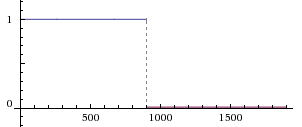
\includegraphics[width=0.7\textwidth]{/graficaGiro.png}
    \caption{Frecuencia de vibración para un giro. El eje vertical indica si está (1) o no (0)
      activo el vibrador, y el eje horizontal indica el tiempo en milisegundos}
    \label{fig:graficaGiro}
  \end{center}
\end{figure}

\begin{figure}[!h]
  \begin{center}
    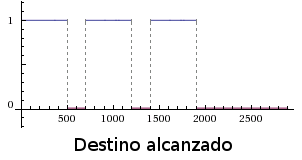
\includegraphics[width=0.7\textwidth]{/graficaDestino.png}
    \caption{Frecuencia de vibración que determina si ha llegado al destino. El eje vertical indica
      si está (1) o no (0) activo el vibrador, y el eje horizontal indica el tiempo en milisegundos}
    \label{fig:graficaDestino}
  \end{center}
\end{figure}

\begin{figure}[!h]
  \begin{center}
    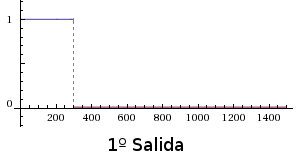
\includegraphics[width=0.7\textwidth]{/graficaRotonda1.png}
    \caption{Frecuencia de vibración para tomar la primera salida de la rotonda. El eje vertical
      indica si está (1) o no (0) activo el vibrador, y el eje horizontal indica el tiempo en
      milisegundos}
    \label{fig:graficaRotonda1}
  \end{center}
\end{figure}

\begin{figure}[!h]
  \begin{center}
    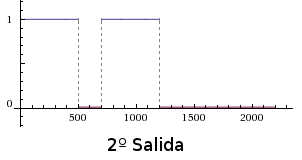
\includegraphics[width=0.7\textwidth]{/graficaRotonda2.png}
    \caption{Frecuencia de vibración para tomar la segunda salida de la rotonda. El eje vertical
      indica si está (1) o no (0) activo el vibrador, y el eje horizontal indica el tiempo en
      milisegundos}
    \label{fig:graficaRotonda2}
  \end{center}
\end{figure}

\begin{figure}[!h]
  \begin{center}
    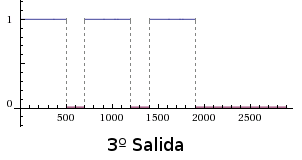
\includegraphics[width=0.7\textwidth]{/graficaRotonda3.png}
    \caption{Frecuencia de vibración para tomar la tercera salida de la rotonda. El eje vertical
      indica si está (1) o no (0) activo el vibrador, y el eje horizontal indica el tiempo en
      milisegundos}
    \label{fig:graficaRotonda3}
  \end{center}
\end{figure}

Una vez que tenemos la forma de codificar las posibles acciones de los complementos vibratorios,
debemos seleccionar qué complementos utilizaremos. En este punto tuvimos un conflicto de
intereses. Tal y como vimos en la sección~\ref{sec:wearables} los únicos complementos que nos
permiten controlar su vibrador a voluntad son los que llevan Android Wear como \acs{SO}, pero estos
dispositivos son muy caros y prácticamente nadie dispone de uno. Por ello, se propuso desarrollar el
proyecto para poder utilizar tanto \emph{wearables} con Android Wear como otros dispositivos con
Android. De este modo podrán utilizar el sistema:

\begin{itemize}
  \item Los usuarios de \textbf{Android Wear} por medio de su \emph{smartphone} y su {wearable}. En
    el teléfono funcionará la aplicación de navegación y se comunicará con el complemento para que
    vibre en los momentos apropiados.

  \item Los usuarios que dispongan de \textbf{dos dispositivos con Android}. En uno funcionará la
    aplicación de navegación y se comunicará con la aplicación del segundo para vibrar en los
    momentos oportunos.

  \item Los usuarios que dispongan de \textbf{un dispositivo Android} en el que se ejecute la
    aplicación principal y \textbf{dos complementos} que vibren en los momentos adecuados. Los
    complementos pueden ser:

    \begin{itemize}
      \item Dos dispositivos con Android
      \item Dos dispositivos con Android Wear
      \item Un dispositivo con Android y otro con Android Wear
    \end{itemize}
\end{itemize}

Para soportar este gran número de configuraciones antes expuesta hacemos uso de la arquitectura
cliente servidor por medio de la tecnología \emph{bluetooth}:

\begin{itemize}
  \item El \textbf{cliente} es la aplicación principal que implementa el sistema de navegación y se
    conecta a los demás dispositivos para hacerlos vibrar de la forma que desee (ver
    cuadro~\ref{cuadro:vibraciones}) y parar la vibración cuando estime oportuno.
  \item Los \textbf{servidores} serán los diferentes dispositivos con Android o Android Wear que
    quedarán a la espera de recibir instrucciones del cliente.
\end{itemize}

De este modo sólo tendremos que implementar en la aplicación de las anteriores iteraciones las
vibraciones del cuadro~\ref{cuadro:vibraciones}, crear una nueva aplicación para Android y otra para
Android Wear que también implemente dichas vibraciones y desarrollar un método de paso de mensajes
por medio de \emph{bluetooth} entre las dos aplicaciones.

\subsubsection{Implementación}

Gracias a que Android y Android Wear comparten gran parte de las \acs{API} podemos utilizar
prácticamente el mismo código para la aplicación del cliente y la aplicación del servidor.

Para poder hacer uso del vibrador de cualquiera de nuestros dispositivos y codificar el
cuadro~\ref{cuadro:vibraciones} hicimos uso de la clase \texttt{Vibrator} que, tras inicializarla,
nos permite manipular el vibrador a voluntad con el método \texttt{vibrate}. De este modo
desarrollamos los métodos \texttt{startLocalVibration} y \texttt{stopLocalVibration} (ver
listado~\ref{code:localVibration}).

\begin{listing}[
  float=ht,
  language = java,
  caption  = {Métodos usados para hacer vibrar el dispositivo con la clase \texttt{Vibrator}},
  label    = code:localVibration]
private void startLocalVibration(int action) {
  if (!mIsInVibration) {
    mIsInVibration = true;
    
    switch (action) {
      case LEFT:
      case RIGHT:
        long[] turn = {0, 900, 1000};
        mVibrator.vibrate(turn, 0);
        break;
		
      case WRONG:
        mVibrator.vibrate(5000);
        break;
				
      case UTURN:
        long[] uturn = {0, 100};
        mVibrator.vibrate(uturn, 0);
        break;
			
      case DESTINATION:
        long[] destination = new long[19];
        for (int i=0; i<3; i++) {
          destination[i*6+1] = 500;
          destination[i*6+2] = 200;
          destination[i*6+3] = 700;
          destination[i*6+4] = 200;
          destination[i*6+5] = 900;
          destination[i*6+6] = 200;
        }
        mVibrator.vibrate(destination, -1);
        break;

      case ROUNDABOUT1:  case ROUNDABOUT2:  case ROUNDABOUT3:
      case ROUNDABOUT4:  case ROUNDABOUT5:  case ROUNDABOUT6:
      case ROUNDABOUT7:  case ROUNDABOUT8:
        int exit = action-20; //roundabout=2X --> x=exit number
        long[] roundabout = new long[exit*2+1];
        for (int i=0; i<exit; i++) {
          if (i != 0) roundabout[i*2] = 200;
            roundabout[i*2+1] = 500;
          }
          roundabout[exit*2] = 1000;
          mVibrator.vibrate(roundabout, 0);
          break;
    }
  } else {
    stopLocalVibration();
    startLocalVibration(action);
  }
}
private void stopLocalVibration() {
  if (mIsInVibration) {
    mVibrator.cancel();
    mIsInVibration = false;
  }
}
\end{listing}

Para establecer una comunicación por \emph{bluetooth} entre el cliente y los servidores utilizamos
la clase \texttt{BluetoothChatService} distribuida en los ejemplos de
Android\footnote{https://developer.android.com/resources/samples/BluetoothChat/index.html}. Esta
clase nos permite abstraernos de la implementación realizada con \texttt{BluetoothSocket} y
centrarnos en qué hacer cuando cambiamos de estado (\emph{escuchando}, \emph{conectando}, etc) o
recibimos un mensaje. Además nos permite iniciar el «chat» y enviar mensajes de forma sencilla.

En la aplicación \textbf{cliente}, que es la que desarrollamos en las iteraciones anteriores,
añadimos un nuevo menú en opciones. Este menú permite activar o desactivar la utilización de la
vibración y, en caso de activarlo, nos permite seleccionar entre los diferentes dispositivos
\emph{bluetooth} emparejados y nuestro dispositivo cuál hará de vibrador derecho y cuál de vibrador
izquierdo. Una vez seleccionado, nuestro cliente intentará iniciar el «chat» con el/los servidor/es
y se quedará a la espera. En caso de no conseguir establecer conexión simplemente avisará al
usuario.

Gracias a utilizar la clase \texttt{BluetoothChatServide}, para iniciar el intercambio de mensajes
sólo es necesario iniciar el servicio con el método \texttt{start} y hacer uso del método
\texttt{connect} proporcionándole el número \acf{MAC} del dispositivo al que queremos
conectarnos. Para definir cómo se comporta la \emph{interfaz} de la aplicación durante el proceso de
conexión hubo que definir un \texttt{Handler} y sobrescribir el método \texttt{handleMesage}
indicando qué hacer mientras se conecta, cuando se desconecte o cuando falle el intento de
conexión. Una vez que estemos conectados podremos enviar mensajes a nuestros dispositivos conectados
por \emph{bluetooth} utilizando los métodos del listado~\ref{code:sendMessage}.

\begin{listing}[
  float=ht,
  language = java,
  caption  = {Métodos utilizados para enviar mensajes por bluetooth haciendo uso de la clase
               \texttt{BluetoothChatServide}},
  label    = code:sendMessage]
private BluetoothChatService mChatServiceLeft = 
    new BluetoothChatService(this, mHandler);
private BluetoothChatService mChatServiceRight =
    new BluetoothChatService(this, mHandler);
private StringBuffer mOutStringBufferLeft = new StringBuffer("");
private StringBuffer mOutStringBufferRight = new StringBuffer("");

[...]

private void sendMessage(String message, int who) {
    if (who == LEFT) {
      sendMessage(message, mChatServiceLeft, mOutStringBufferLeft);
    } else if (who == RIGHT) {
      sendMessage(message, mChatServiceRight, mOutStringBufferRight);
    }
}

private void sendMessage(String message, BluetoothChatService d, StringBuffer b) {
    if (d == null || d.getState() != BluetoothChatService.STATE_CONNECTED) {
        return;
    }
    	
    message = message + SPLIT;
    if (message.length() > 0) {
        byte[] send = message.getBytes();
        d.write(send);
        b.setLength(0);
    }
}
\end{listing}

Para el caso de los \textbf{servidores} desarrollamos dos aplicaciones: una para Android y otra para
Android Wear. En ambas aplicaciones iniciamos el servicio \texttt{BluetoothChatService} al ejecutar
la aplicación quedándonos a la escucha de conexiones \emph{bluetooth}. Además definimos un
\texttt{Handler} para especificar qué hacer en los diferentes estados de la conexión con la
\emph{interfaz} y determinar qué hacer en caso de recibir un mensaje (ver
listado~\ref{code:servidorHandler}).

\begin{listing}[
  float=ht,
  language = java,
  caption  = {Métodos utilizados en los servidores para leer los mensajes recibidos por medio de de
               la clase \texttt{BluetoothChatServide} },
  label    = code:servidorHandler]
private Handler mHandler = new Handler() {
  public void handleMessage(Message msg) {
    switch (msg.what) {
      case BluetoothChatService.MESSAGE_STATE_CHANGE:
        switch (msg.arg1) {
          case BluetoothChatService.STATE_CONNECTING:
          case BluetoothChatService.STATE_LISTEN:
          case BluetoothChatService.STATE_NONE:
            [...]
            break;
          case  BluetoothChatService.STATE_DISCONNECTING:
            [...]
            break;
        }
        break;

      case BluetoothChatService.MESSAGE_READ:
        byte[] readBuf = (byte[]) msg.obj;
        String readMessages = new String(readBuf, 0, msg.arg1);
        String readMessage = "";
                
        for (int i=0; i<readMessages.length(); i++) {
          if (readMessages.charAt(i) == SPLIT) {
            startAction(readMessage);
            readMessage = "";
          } else {
            readMessage = readMessage + readMessages.charAt(i);
          }
        }
        break;

      [...]
    }
  }
};

private void startAction (String readMessage) {
  if (readMessage.equals(STOP)) {
    stopLocalVibration();
  } else if (readMessage.length() > 1) {
    stopLocalVibration();
    int action = Integer.parseInt(readMessage.substring(1));
    startLocalVibration(action);
  }
}
\end{listing}

Como se puede apreciar en los listados \ref{code:sendMessage} y \ref{code:servidorHandler} a la hora
de intercambiar mensajes incluimos un separador: \texttt{SPLIT}. Esto se debe a que durante el
desarrollo del intercambio de mensajes se detectaron errores se sincronización entre los
\texttt{buffers} del cliente y de los servidores. De este modo nos aseguramos de no malinterpretar
los mensajes.

\subsubsection{Pruebas}

Al finalizar la implementación del noveno prototipo se realizó la siguiente prueba:

\begin{itemize}
  \item Para determinar el correcto funcionamiento de la vibración y del paso de mensajes

  \begin{tabular}{p{.15\textwidth}p{.75\textwidth}}
    \hline
    \textbf{Dado}     & Diferentes rutas \\
                      & Diferentes dispositivos con distintas versiones de Android \\
                      & Diferentes formas posibles de conectar dichos dispositivos:
                        Android-Android, Android-Android Wear, Android-Android-Android y 
                        Android-Android-Android Wear \\
                      & Todas las posibles acciones de guiado \\
    \textbf{Cuando}   & Debemos realizar alguna acción \\
    \textbf{Entonces} & Vibra el dispositivo adecuando con la frecuencia correspondiente a
                        la acción a realizar \\
    \hline
  \end{tabular}
\end{itemize}

% Local Variables:
% TeX-master: "main.tex"
%  coding: utf-8
%  mode: latex
%  mode: flyspell
%  ispell-local-dictionary: "castellano8"
% End:
